% Emacs settings: -*-mode: latex; TeX-master: "manual.tex"; -*-

\chapter{Beam optical components:
Arms, slits, collimators, and filters}
This chapter contains a number of optical components
that is used to modify the neutron beam in various ways,
as well as the ``generic'' component \textbf{Arm}.
\index{Library!Components!optics}
\index{Optics|textbf}

\section{Arm: The generic component}
\label{s:arm}
\index{Optics!Point in space (Arm, Optical bench, Coordinate system)}
\mcdoccomp{optics/Arm.parms}

The component \textbf{Arm} is empty; is resembles an optical bench
and has no effect on the x-ray.
The purpose of this component is only to provide a standard
means of defining a local coordinate system within the instrument definition.
Other components may then be
positioned relative to the \textbf{Arm} component
using the \MCX\ meta-language.
The use of \textbf{Arm} components in beamline definitions
is not required but is recommended for clarity.
\textbf{Arm} has no input parameters.

The first Arm instance in an instrument definition may be changed into a
\textbf{Progress\_bar} (sec.~\ref{s:progress-bar}) component in order to display
simulation progress on the fly, and possibly save intermediate results.


\section{Slit: A beam defining diaphragm}
\label{slit}
\index{Optics!Slit}

%\component{Slit}{System}{$x_\textrm{min}$, $x_\textrm{max}$, $y_\textrm{min}$, $y_\textrm{max}$}{$r$, $p_\textrm{cut}$}{}
\mcdoccomp{optics/Slit.parms}

The component \textbf{Slit} is a very simple construction.
It sets up an opening at $z=0$, and propagates the neutrons
onto this plane (by the kernel call PROP\_Z0).
Neutrons within the slit opening are unaffected,
while all other neutrons
are discarded by the kernel call ABSORB.

By using \textrm{Slit}, some neutrons contributing to the background
in a real experiment will be neglected.
These are the ones that scatter off the inner side
of the slit, penetrates the slit material,
or clear the outer edges of the slit.

The input parameters of \textbf{Slit} are the four coordinates,
$(x_\textrm{min}, x_\textrm{max}, y_\textrm{min}, y_\textrm{max})$
defining the opening of the rectangle, or the radius $r$ of
a circular opening, depending on which parameters are specified.

The slit component can also be used to discard insignificant 
({\em i.e.}\ very low weight)
neutron rays, that in some simulations may be very abundant and therefore
time consuming. If the optional parameter $p_\textrm{cut}$ is set, all
neutron rays with $p<p_\textrm{cut}$ are ABSORB'ed.
This use is recommended in connection with \textbf{Virtual\_output}.




\section{Beamstop: A photon absorbing area}
\label{beamstop}
\index{Optics!Beam stop}

\mcdoccomp{optics/Beamstop.parms}

The component \textbf{Beamstop} can be seen as the reverse of
the \textbf{Slit} component.
It sets up an area at the $z=0$ plane. Photons that hit the plane 
within this area are ABSORB'ed, while all others are unaffected.

By using this component, some photons contributing to the background
in a real experiment will be neglected.
These are the ones that scatter off the side
of the (real) beamstop, or penetrate the absorbing material.
Further, the holder of the beamstop is not simulated.

\textbf{Beamstop} can be either circular or rectangular.
The input parameters of \textbf{Beamstop} are either height and width \textit{(xwidth, yheight)} or the four coordinates,\textit{(xmin, xmax, ymin, ymax)}
defining the opening of a rectangle, or the \textit{radius} of
a circle, depending on which parameters are specified.

If the "direct beam" (e.g. after a monochromator or sample) should not be
simulated, it is possible to emulate an ideal beamstop 
so that only the scattered beam is left;
without the use of \textbf{Beamstop}:
This method is useful for instance in the case where only photons 
scattered from a sample are of interest. 
The example below removes the direct beam and 
any background signal from other parts of the beamline
\begin{verbatim}
COMPONENT MySample=PowderN(...) AT (...)
EXTEND
%{
  if (!SCATTERED) ABSORB;
%}
\end{verbatim}


\section{Filter: A general absorption filter model}
\label{s:filter}
\index{Optics!Filter}
\mcdoccomp{optics/Filter.parms}

This component is a filter in the shape of a rectangular block or a general
shape defined by a set of polygons. Given an input file containing material
parameters. Neccessary parameters are nominal density and a parameterization of
the linear attenuation coefficient, $\mu$ as a function of wavelength (or
energy).

The model is very simple: Firstly the X-ray is traced to find intersection points between ray and filter (0 or 2).
If no intersection is found the x-ray is left untouched and nothing further happens.
Assuming the ray intersects the filter: Secondly, the path length d$l$ within the filter is computed.
Thirdly a $\mu = f(\lambda,\mathrm{material})$ is computed by interpolating in
a datafile, and the x-ray weight is adjusted according to
$p=p\exp(-\mathrm{d}l*\mu)$. The x-ray is left at the point where it exits the
filter block (the $2$nd intersection).

Example data files corresponding to all elements up to $Z=92$ are distributed with \MCX in the
\verb+MCXTRACE/data+ directory as \verb+*.txt+ files. These tables have been
extracted from the NIST FFAST~\cite{NIST-ffast} x-ray database.
To generate other datafiles from the same source a simple shell script:
\verb+MCXTRACE/data/get_xray_db_data+ is also distributed with \MCX
Running this script will connect to the NIST webiste and download a
\verb+.html+ file. This output must now be modified such that \verb+html+-tags
are removed and all header lines begin with $\#$

\subsection{Example}
\label{getNISTdata}
This is an example of how to download and generate datafiles for the \verb+Filter.comp+ and others.

The distributed tables have been extracted from the NIST x-ray database. To ease generation of more dtafiles
from the same source a simple shell script:\\
\verb+MCXTRACE/data/get_xray_db_data+\\
is also distributed with \MCX

Running this script will connect to the NIST webiste and download a \verb+.html+ file. This output must now be modified wuch that \verb+html+-tags
are removed and all header lines begin with $\#$.

\begin {verbatim}
 /usr/local/lib/mcxtrace/data/get_xray_db_data 3 output.dat
\end{verbatim}
where the second parameter (3) is the atom number of the material, for which we want to generate a datafile.
Now open the generated datafile (\verb+output.dat+) with your favourite text editor and make sure the file ends up looking like this
\tiny
\begin{verbatim}
#Li (Z 3)
#Atomic weight: A[r]  6.941000
#Nominal density: rho 5.3300E-01
#    rho[a](barns/atom) = [mu/rho](cm^2 g^-1)  x  1.15258E+01
#    E(eV) [mu/rho](cm^2 g^-1) = f[2](e atom^-1)  x  6.06257E+06
#    2 edges. Edge energies (keV):
#
#
#    K      5.47500E-02  L I    5.34000E-03
#
#Relativistic correction estimate f[rel] (H82,3/5CL) = -9.8613E-04,
#    -6.0000E-04 e atom^-1
#    Nuclear Thomson correction f[NT] = -7.1131E-04 e atom^-1
#
#-------------------------------------------------------------------------------
#Form Factors, Attenuation and Scattering Cross-sections
#Z=3, E = 0.001 - 433 keV
#
#    E        f[1]         f[2]        [mu/rho]    [sigma/rho]  [mu/rho]   [mu/rho][K] lambda
#                                    Photoelectric Coh+inc      Total
#   keV        e atom^-1    e atom^-1   cm^2 g^-1   cm^2 g^-1   cm^2 g^-1   cm^2 g^-1  nm
5.233200E-03  9.08733E-01  0.0000E+00  0.0000E+00  2.3914E-07  2.3914E-07  0.000E+00  2.369E+02
5.313300E-03  8.59283E-01  0.0000E+00  0.0000E+00  2.5404E-07  2.5404E-07  0.000E+00  2.333E+02
5.334660E-03  8.03599E-01  0.0000E+00  0.0000E+00  2.5813E-07  2.5813E-07  0.000E+00  2.324E+02
5.366700E-03  8.56971E-01  1.0769E-01  1.2165E+05  2.6435E-07  1.2165E+05  0.000E+00  2.310E+02
.
.
.
3.788588E+02  3.00000E+00  3.9121E-08  6.2602E-07  8.4389E-02  8.4390E-02  6.123E-07  3.273E-03
4.050001E+02  3.00000E+00  3.3438E-08  5.0054E-07  8.2127E-02  8.2128E-02  4.895E-07  3.061E-03
4.329451E+02  3.00000E+00  2.8581E-08  4.0022E-07  7.9892E-02  7.9892E-02  3.913E-07  2.864E-03
\end{verbatim}
\normalsize
Please make sure you don't forget to remove the html-tags in the bottom of the file as well. In the future we will set
up a more streamlined way of doing this.


\newpage
\input{optics/Collimator_linear}

\input{optics/Collimator_radial}

\newpage
\chapter{Reflecting optical components: mirrors, and guides}
\index{Optics|textbf}

This section describes advanced neutron optical
components such as supermirrors and guides as well as various rotating choppers.
A description of the reflectivity of a supermirror is found
in section~\ref{s:mirror}.

\input{optics/Guide}

\chapter{Moving optical components:
Choppers and velocity selectors}
We list in this chapter some moving optical components,
like choppers, that may be used for TOF class instrument simulations,
and velocity selector used for partially monochromatize continuous beams.
\index{Library!Components!optics}
\index{Optics|textbf}

\input{optics/DiskChopper}

\newpage
\section{FermiChopper: The Fermi-chopper}

\component{FermiChopper}{M. Poehlmann, C. Carbogno, H. Schober, E. Farhi}{$R,y_{min} y_{max}, \nu,w,length$,Nslit,phase}{$m,Q_c,R_0,\alpha, W$,curvature,zero\_time}{validated}
\index{Optics!Fermi Chopper|textbf}

\begin{figure}
\begin{center}
\begin{tabular}{cc}
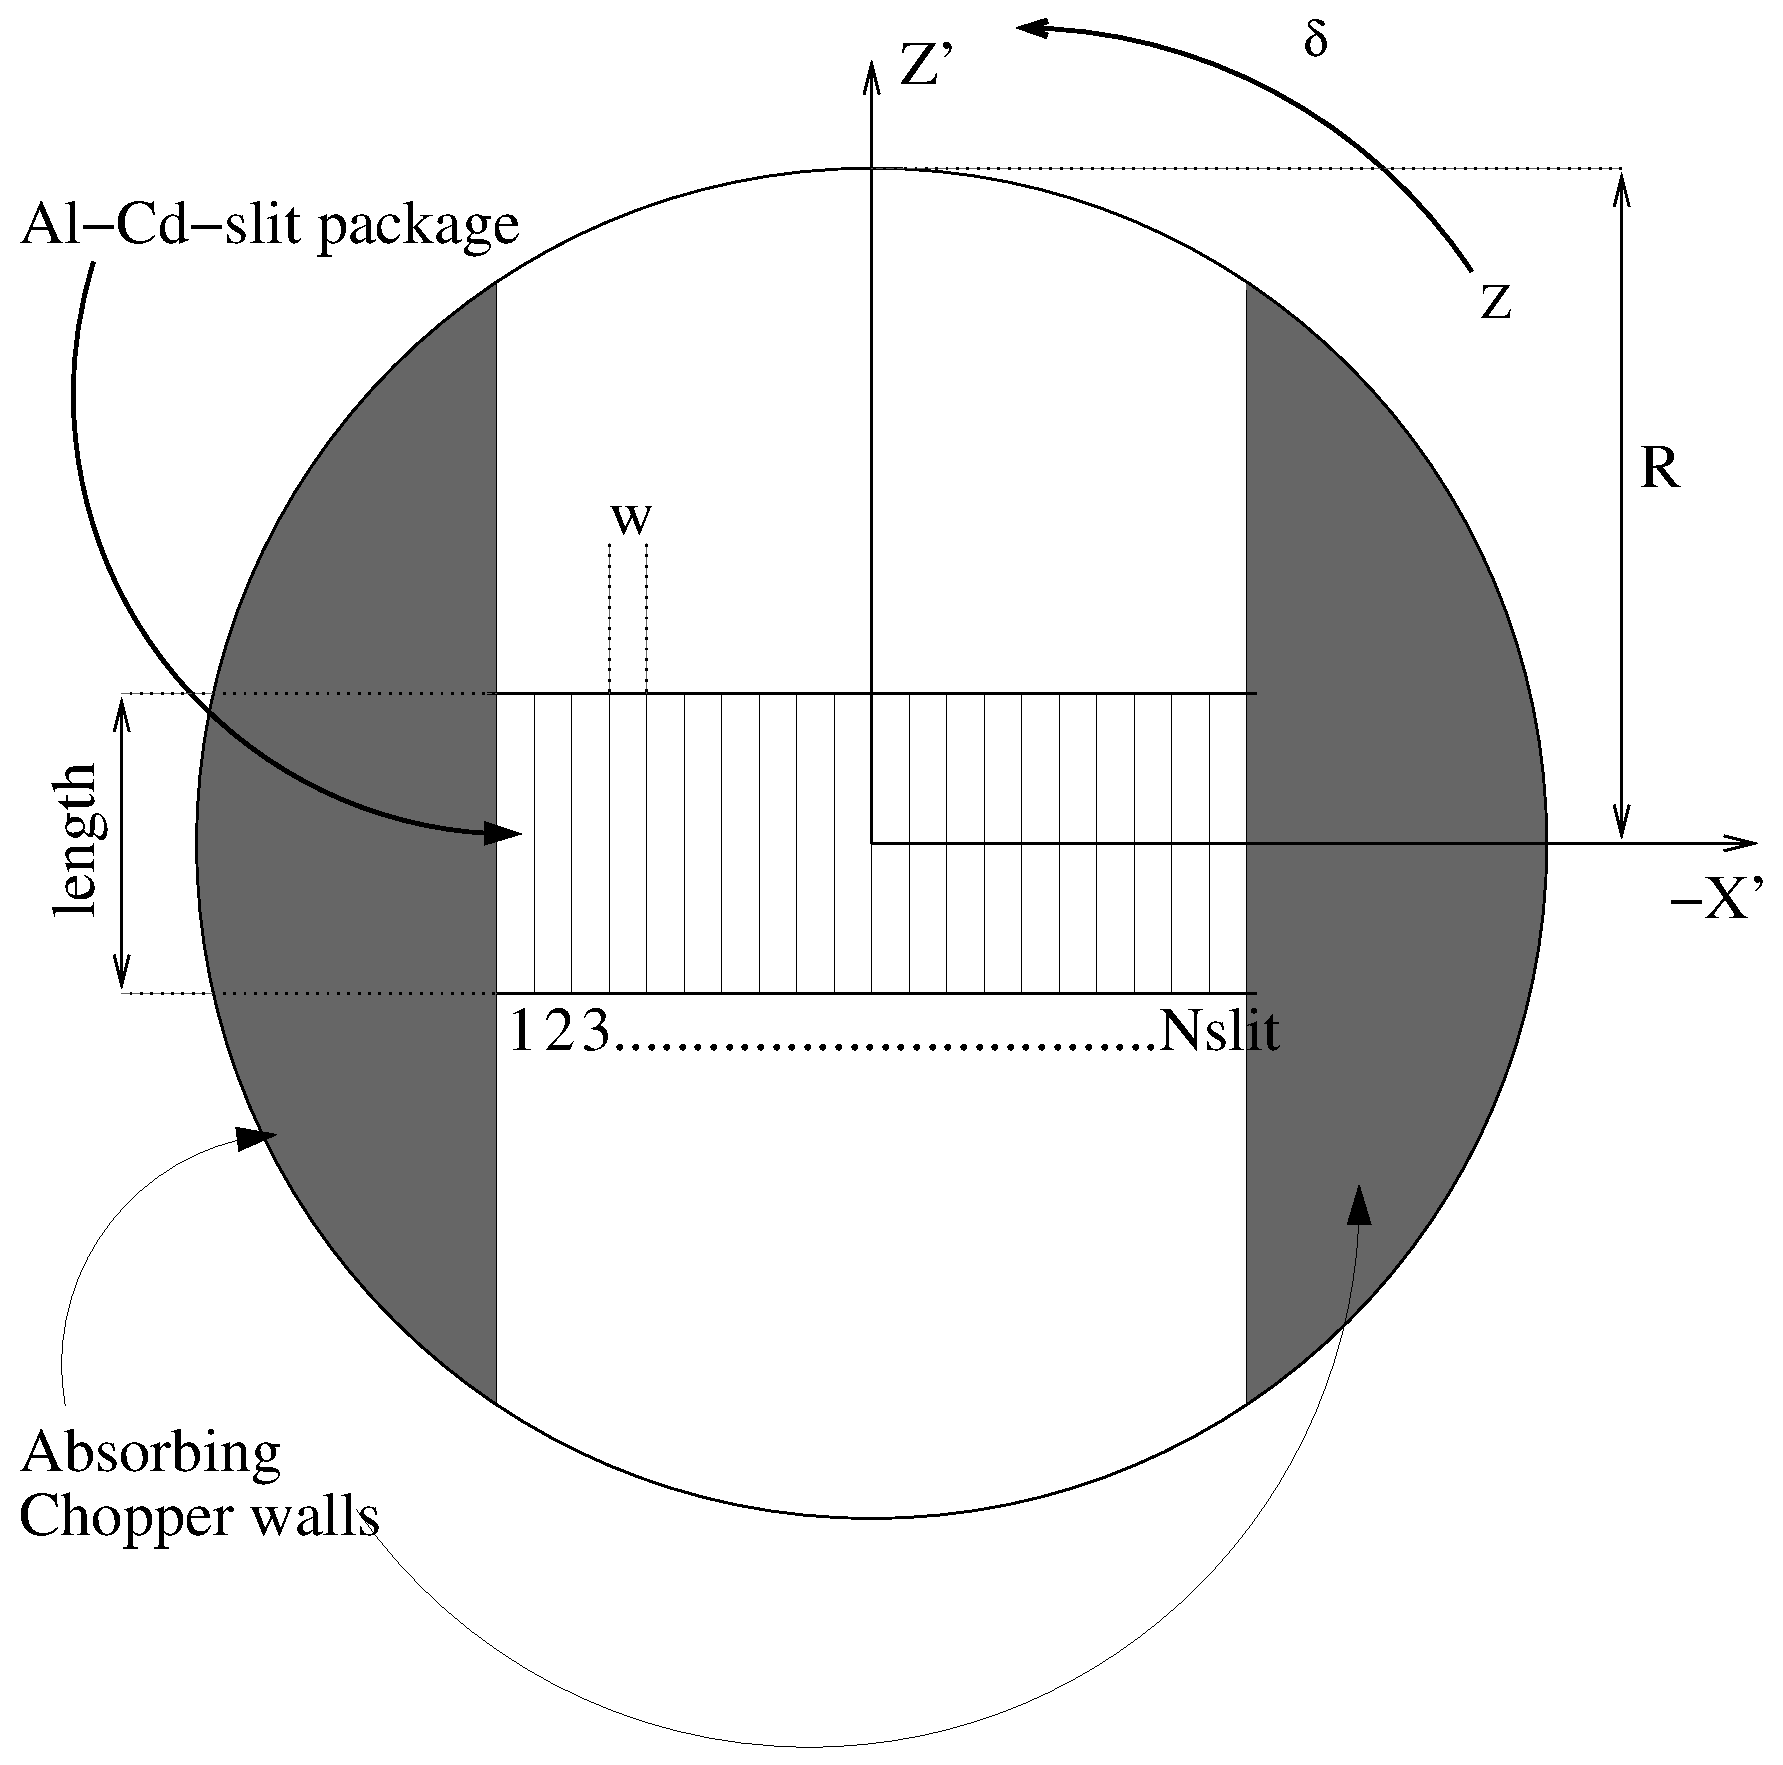
\includegraphics[height=7cm]{./figures/FCChoppergeo.eps}
&
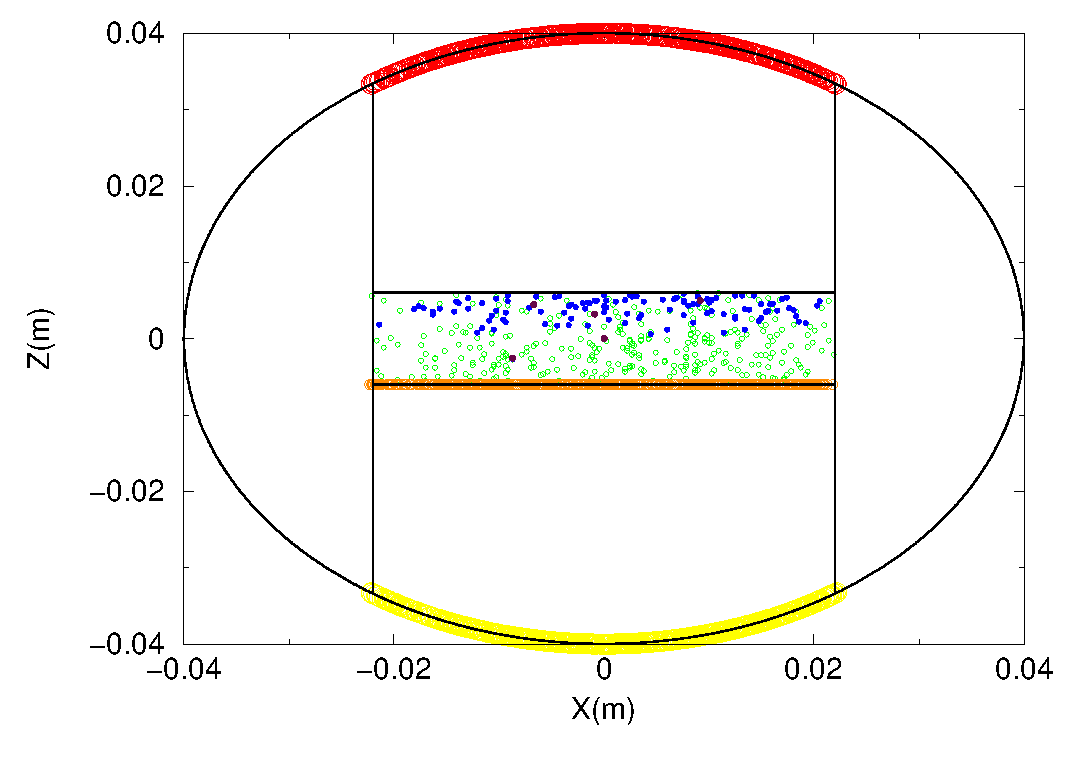
\includegraphics[height=5cm,width=5.3cm]{./figures/FCOverview.eps}
\end{tabular}
\end{center}
\caption{Geometry of the Fermi-chopper (left) and Neutrons in the chopper (right).}
\label{fig:Overview.eps}
\end{figure}

\subsection{The chopper geometry and parameters}
\label{ssec:chopper}

The Fermi chopper is a rotating vertical cylinder containing a set of collimating slits (\emph{slit package}). Main geometry parameters are the radius $R$, minimum and maximum height $y_{min}$ and $y_{max}$ (see Fig. \ref{fig:Overview.eps}).
In this implementation, the slits are by default straight, but may be coated with super-mirror, and curved. Main parameters for the slits are the number of slits $Nslit$, the length $length$ and width $w$ of each slit, the width of the separating Cd-blades is neglected. The slit walls reflectivity is modelled just like in guide components by the $m$-value ($m > 1$ for super mirrors), the critical scattering vector $Q_c$, the slope of reflectivity $\alpha$, the low-angle reflectivity $R_0$ and the width of supermirror cut-off $W$. For $m=0$ the blades are completly absorbing. The AT position of the component is its center.

The angular speed of the chopper is $\omega = 2\pi \nu$, where $\nu$ is the rotation frequency. The angle $phase$ for which the chopper is in the 'open' state for most of the neutrons coming in (z' axis of the rotating frame parallel to the z axis of the static frame) is also an input parameter. The time window may optionally be shifted to zero when setting the \verb+zero_time=1+ option. A phase guess value may be set automatically using the \verb+zero_time=2+ option.

The curvature of the slit channels is specified with the {\it curvature} parameter. Positive sign indicates that the deviation 'bump' due to curvature is in the $x'$ positive side, and the center of curvature is in the $x'$ negative side. The optimal radius of curvature $R$ is related to frequency $\nu$ and neutron velocity $v$ with: $v=4 \pi R \nu$.

The component was validated extensivelly by K. Lieutenant. As an alternative, one may use the {\bf Vitess\_ChopperFermi} component (eventhough slower and without super-mirror support) or the {\bf FermiChopper\_ILL} contributed component. The Guide\_gravity component has also a rotating mode, using an approximation of a Fermi Chopper.

\begin{table}
  \begin{center}
  {\let\my=\\
    \begin{tabular}{|lr|p{0.6\textwidth}|}
    \hline
Parameter & unit & meaning \\
    \hline
radius & [m] & chopper cylinder radius \\
ymin   & [m] &   lower y bound of cylinder \\
ymax   & [m] &   upper y bound of cylinder \\
Nslit  & [1] &   number of chopper slits \\
length & [m] &   channel length of the Fermi chopper \\
w      & [m] &   width of one chopper slit. May also be specified as \emph{width}=w*Nslit for total width of slit package. \\
nu & [Hz] &  chopper frequency \\
phase     & [deg] &   chopper phase at t=0 \\
zero\_time & [1] & shit time window around 0 if true \\
curvature & [m$^{-1}$] & Curvature of slits (1/radius of curvature) \\
    \hline
m     & [1] & \\
alpha & [\AA] & \\
Qc    & [\AA$^{-1}$] & slit coating parameters. See section \ref{ss:mirrorreflect} \\
W     & [\AA$^{-1}$] & \\
R0    & [1] & \\
    \hline
    \end{tabular}
    \caption{FermiChopper component parameters}
    \label{t:fc-param}
  }
  \end{center}
\end{table}


\subsection{Propagation in the Fermi-chopper}

As can be seen in figure \ref{fig:Overview.eps}, neutrons first propagate onto the cylinder surface of the chopper (yellow curve). Then the program checks the interaction with the entrance of the slit package (orange line) and calculates which slit is hit. If the slit coating is reflecting ($m > 0$), multiple reflections are calculated (green, blue and maroon circles), otherwise the neutrons are absorbed as soon as they interact with the blades. Finally the remaining neutrons propagate to the exit of the chopper (red curve).

The rotation of the chopper is characterized by the angle $\delta$ between the rotating z' and the static z-axis. $\delta(t)$ is defined by:

$$\delta(t) = \widehat{z,z'} = \omega.(t-t_0) = \omega.t+\phi_0$$

where $t$ is the absolute time, $t_0$ is the chopper delay, and $\phi_0$ is the chopper phase. The chopper should better be \emph{time focussing}: slow neutrons should pass before the fast ones, so that they finally hit the detectors at the same time. Therefore the signs of $\omega$ and $\delta$ are very important: For $t>t_0$, $\delta$ is positive and points anti-clockwise.

Since the rotation is applied along the y - axis, we can simplify the problem to two dimensions. The orthogonal transformation matrix $T$ from the static $(zx)$ to the rotating frame $(z'x')$ is:
\begin{equation}
T_{zx \rightarrow z'x'} = \left(
\begin{array}{cc}
\cos(\delta) & \sin (\delta) \\
-\sin(\delta) & \cos(\delta)
\end{array}
\right)
\end{equation}

\begin{figure}
\begin{center}
\begin{tabular}{cc}
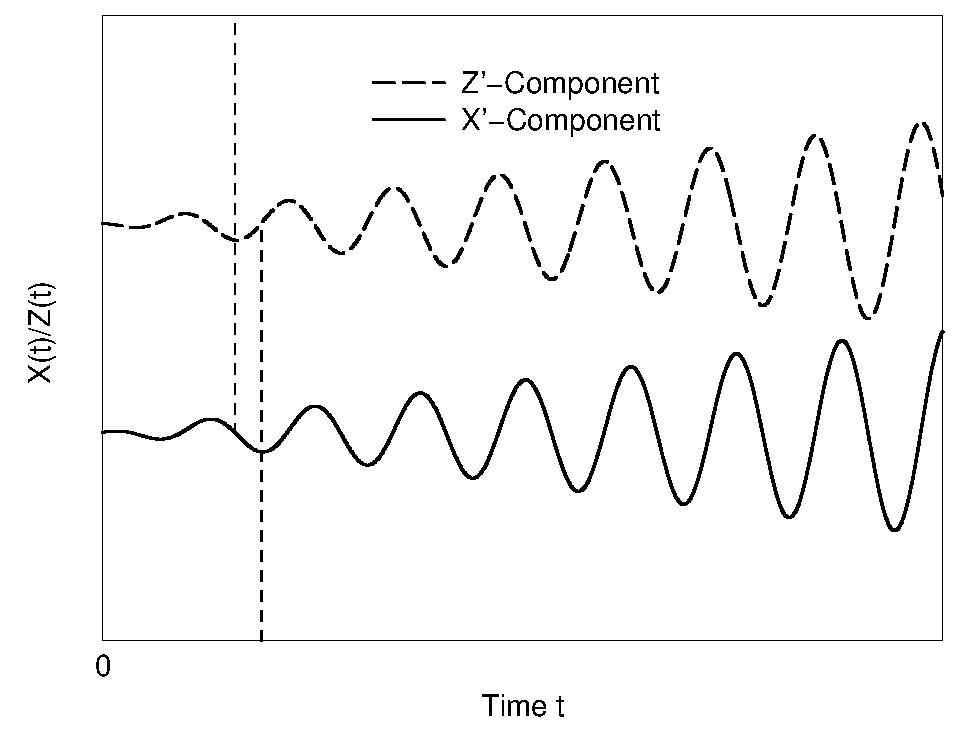
\includegraphics[height=5.5cm]{./figures/XZCoords.eps}
&
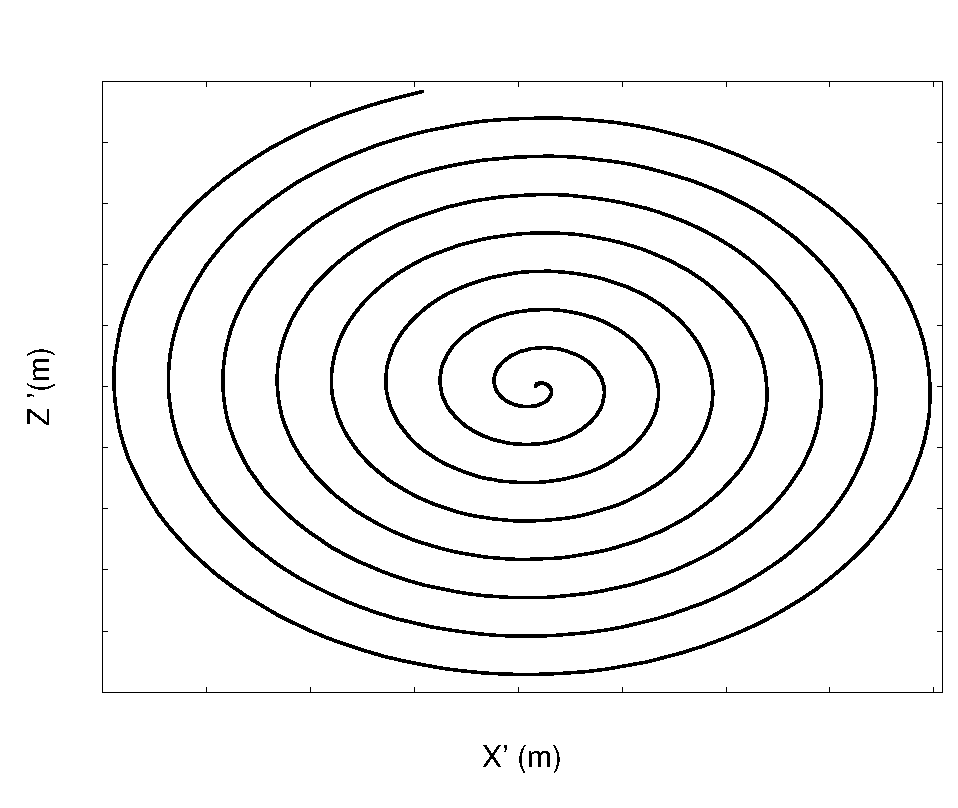
\includegraphics[height=6.5cm,width=5.5cm]{./figures/XZplain.eps}
\end{tabular}
\end{center}
\caption{The x' and z' component as a function of time in the rotating frame (left). A typical neutron trajectory in the rotating frame (right).}
\label{fig:Component.eps}
\end{figure}

Together with the equation for a non-accelerated, linear propagation $\vec{r} = \vec{r_0}+\vec{v}t$ the orthogonal transformation produces a curve in the Z'-X'-plane known as \emph{archidemic spiral}, as can be seen in figure \ref{fig:Component.eps}. The two vector components $s(t) = (z',x')$ follow the equation:
\begin{equation}
s(t) = \left(
\begin{array}{c}
z' \\
x'
\end{array}
\right) = T.\left(
\begin{array}{c}
z(t) \\
x(t)
\end{array}
\right) = \left(
\begin{array}{c}
(z_0+v_z.t)cos(\delta(t)) + (x_0+v_x.t)sin(\delta(t)) \\
-(z_0+v_z.t)sin(\delta(t)) + (x_0+v_x.t)cos(\delta(t))
\end{array}
\right).
\label{eq:Txz}
\end{equation}
For a fixed chopper rotation speed, the neutron trajectory tends to strech from a spiral curve for slow neutrons to a straight line for fast neutrons. For real Fermi chopper settings $\nu$ (about 100 Hz on IN6 at the ILL), neutron trajectories are found to be nearly straight for 1000 m/s neutron velocities \cite{blanc83}.

The basis of the algorithm is to find the intersections of these spiral trajectories with the chopper outer cylinder and then the slit package, in the rotating frame.

For this purpose, the \emph{Ridders's} root finding method was implemented \cite{NumRecip} in order to solve
\begin{equation}
x'(t) = d {\rm\ or\ } z'(t) = d
\label{eq:Ridder}
\end{equation}
This method provides faster and more accurate intersection determination than other common algorithms. E.g. the secant method fails more often and may give wrong results (outside chopper) whereas the bisection method (a.k.a Picard dichotomy) is slightly slower.

\subsubsection{Standard slit packages (non super-mirror)}

\begin{figure}
\begin{center}
\begin{tabular}{cc}
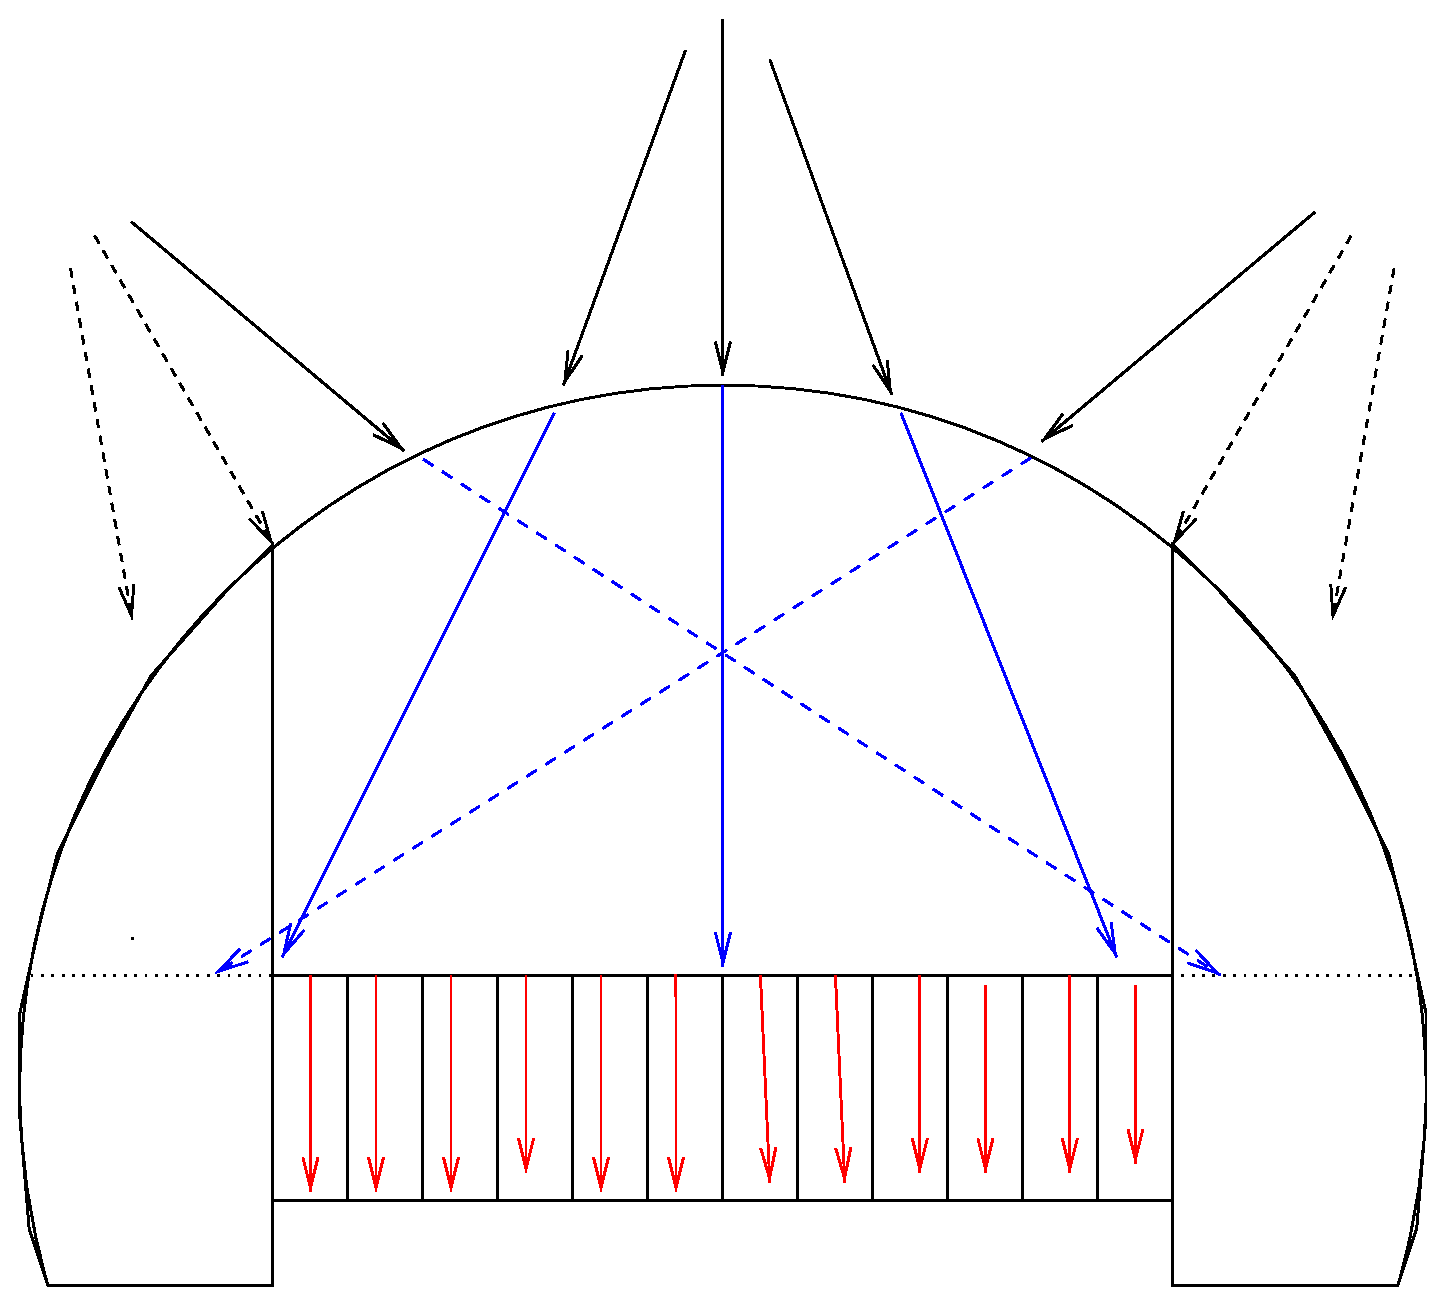
\includegraphics[height=5cm]{./figures/FCAlgo.eps}
&
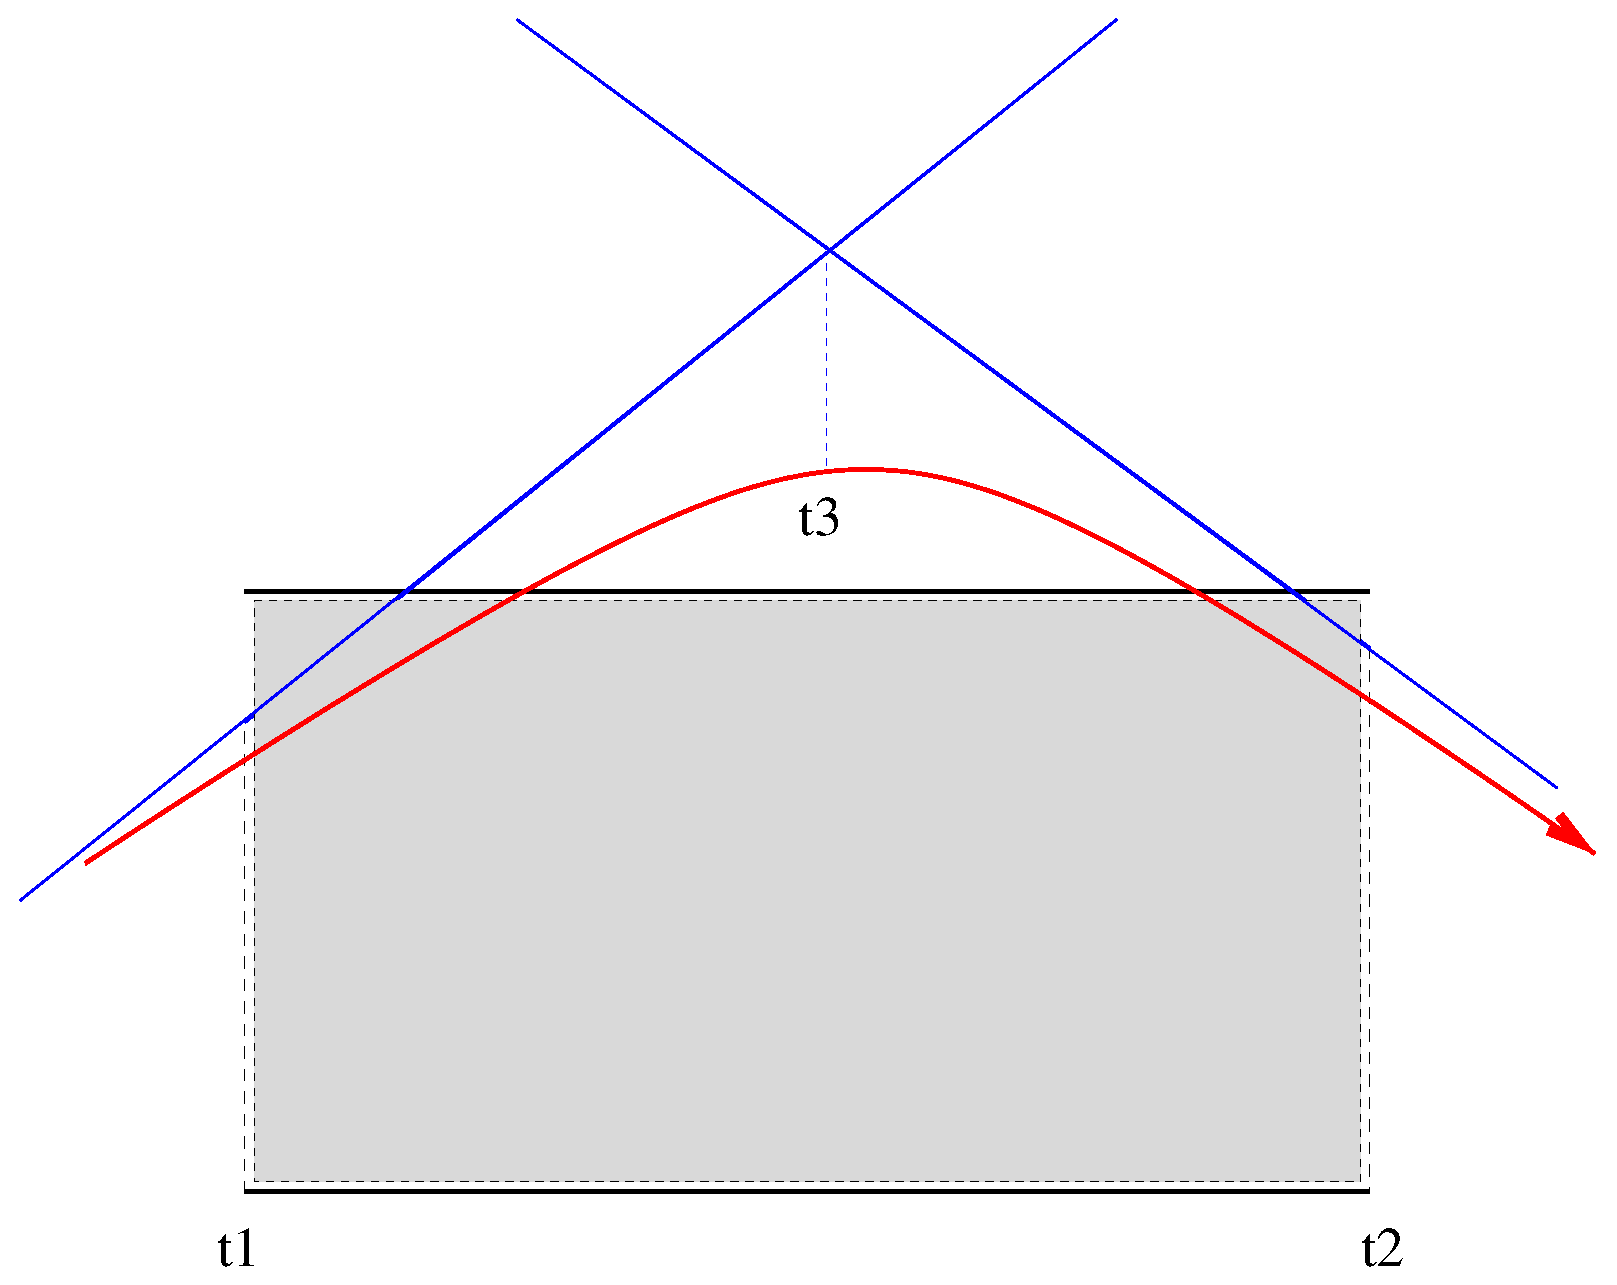
\includegraphics[height=5cm]{./figures/FCtangents.eps}
\end{tabular}
\end{center}
\caption{The different steps in the algorithm (left). A neutron trajectory in a slit (right)}
\label{fig:TOFalg.eps}
\end{figure}

The neutrons are first propagated to the outer chopper cylinder and their coordinates are transformed into the rotating frame using $T$. Neutrons outside the slit channel (chopper opening), or hitting the top and bottom caps are absorbed (yellow dots in Fig. \ref{fig:Overview.eps}). The side from which the neutron approaches the chopper is known (positive or negative z'-axis of the rotating frame) so that the calculation of the time of interaction with the slit package entrance $t_1$ is performed solving $z' = \pm \frac{\rm length}{2}$ in Eq. (\ref{eq:Txz}). Using the result of the numerical algorithms the neutron propagates to the entrance of the slit package (orange circles in Fig. \ref{fig:Overview.eps}). Neutrons getting aside the slit package entrance are absorbed. Additionally, the slit package exit time $t_2$ is estimated the same way with $z' = \mp \frac{\rm length}{2}$, in order to evaluate the whole time-of-flight in the chopper. The index of the slit which was hit is also computed, as we know the $x'$ coordinate in the rotating frame at the slit entrance.

Differentiating Eq. (\ref{eq:Txz}) for $x$ coordinate
\begin{equation}
\dot{x'}(t) = v_x'(t) = [v_x-\omega.(z+v_z.t)]\cos(\omega(t-t_0)) - [v_z+\omega.(x+v_x.t)]\sin(\omega(t-t_0))
\end{equation}
we may estimate the tangents to the spiral neutron trajectory in the rotating frame at times $t_1$ and $t_2$. The intersection of these two lines gives an intermediate time $t_3$.

If the neutron remains in the same slit at this point, then there is no intersection with the slit walls (direct flight), and the neutron may be propagated to the slit output, and then to the cylinder output. A last check is made for the neutron to pass the chopper aperture in the cylinder.

If the neutron changes of slit channel at this point, we may determine the intersection time of the neutron trajectory within $[ t_1, t_3 ]$ or $[ t_3, t_2 ]$, as seen in Fig. \ref{fig:TOFalg.eps}. If walls are not reflecting, we just absorb neutrons here.

\subsubsection{The reflections (super-mirror slits)}

If slit walls are reflecting, neutron is first propagated to the slit separating surface. Then the velocity in the rotating frame is computed using Eq. (\ref{eq:Txz}). Perpendicular velocity $v_x'$ is reverted for reflection, and inverse $T$ transformation is performed. Reflected intensity is computed the same way as for the guide component (see section \ref{s:mirror}). The remaining time $t_2$ to the slit output is estimated and the tangent intersection process is iterated, until neutron exits. Remember that super mirror $m < 1$ parameters behave like $m=1$ materials (see section \ref{ss:mirrorreflect}). Selecting $m=0$ sets the blabes absorbing.

The propagation is finalized when determining the intersection of the neutron trajectory with the outer surface of the chopper cylinder. The neutron must then pass its aperture, else it is absorbed.

\subsubsection{Curved slit packages}

The effect of curvature can significantly improve the flux and energy resolution shape.

As all $(zx)$ cordinates are transformed into $(z'x')$, the most efficient way to take into account the curvature is to include it in the transformation Eq. (\ref{eq:Txz}) by 'morphing' the curved rotating real space to a straight still frame. We use parabolic curvature for slits. Then instead of solving
\begin{equation}x'(t) = d - \Delta_{x'}(z') {\rm\ where\ } \Delta_{x'}(z')=R_{slit}.(1-\sqrt{1-(z'/R_{slit})^2})
\end{equation}
with $\Delta$ being the gap between the straight tangent line at the slit center and the real slit shape, we perform the additional transformation
\begin{equation}
x' \rightarrow x' + \Delta_{x'}(z')
\end{equation}
The additional transformation counter-balances the real curvature so that the rest of the algorithm is written as if slits were straight.
This applies to all computations in the rotating frame, and thus as well to reflections on super mirror coatings.



% Emacs settings: -*-mode: latex; TeX-master: "manual.tex"; -*-

\section{Vitess\_ChopperFermi: The Fermi Chopper from Vitess}
\label{s:vit_fc}
\index{Optics!Fermi Chopper}

\component{Vitess\_ChopperFermi}{Geza Zsigmond}{GeomOption, $N_{\rm chan}$, $f$, $h$, $w_{\rm tot}$, $l$, $r_{\rm curv}$, $d$, $\phi$, $w_{\rm wall}$, GeomFile}{zerotime, $N_{\rm gates}$}{validated}


The component {\bf Vitess\_ChopperFermi} simulates a Fermi chopper with absorbing walls.
The shape of the channels can be straight, curved with circular, or curved with ideal
(i.e. close to a parabolic) shape.
This is determined by the parameter 'GeomOption'. In the option 'straight Fermi
chopper', the very fast neutrons are transmitted with only a time modulation and lower
speed neutrons are modulated both in time of flight and wavelength.
If the channels are curved, the highest transmission occurs for a wavelength

\begin{equation}
\lambda_{\rm opt} = \frac{3956 {\rm [m\AA/s]}}{2 \omega r_{\rm curv}}
\end{equation}

with

\begin{equation}
\omega = 2 \pi f
\end{equation}

The optimal shape is calculated in an exact way and is close to parabolic; in this
case, transmission is as high for the optimal wavelength as in the case of a straight
Fermi chopper for the limit $\lambda \rightarrow 0$.
In the more realistic case of circular shapes channels, the transmission is slightly
lower. In general, neutrons are transmitted through a curved Fermi chopper with a time
AND wavelength modulation .

The rotation axis is vertical (y-axis), i.e. the path length through the channels is
given by the length $l$ along the z-axis. The inital orientation is given by the phase
$\phi$ of the chopper - $\phi$ = 0 means transmission orientation.

Geometry for {\bf straight} and {\bf circular} channels:
The geometry of the chopper consists of a rectangular shaped object with a channel
system. In transmission position, there are $N_{\rm gates}$ slits of width $w_{\rm slit}$
each along the x-axis, separated by absorbing walls of thickness $w_{\rm wall}$
(see figure~\ref{f:vit_fc1}). The total width $w_{\rm tot}$ is given by

\begin{equation}
w_{\rm tot} = N_{\rm gates} w_{\rm slit} + (N_{\rm gates}+1) w_{\rm wall}
\end{equation}

The rectangular channel system is surrounded by a so-called shadowing cylinder; it is a
part of a cylinder with vertical symmetry axis and diameter

\begin{equation}
d \geq \sqrt{l^2 + w_{\rm tot}^2}
\end{equation}

It serves to prevent transmission of neutrons which do not fly through the channels;
but it also reduces the transmission, because the cylinder removes neutrons
in front of the channel entrance or behind the channel exit (see figure~\ref{f:vit_fc1}).

\begin{figure}[ht]
\begin{center}
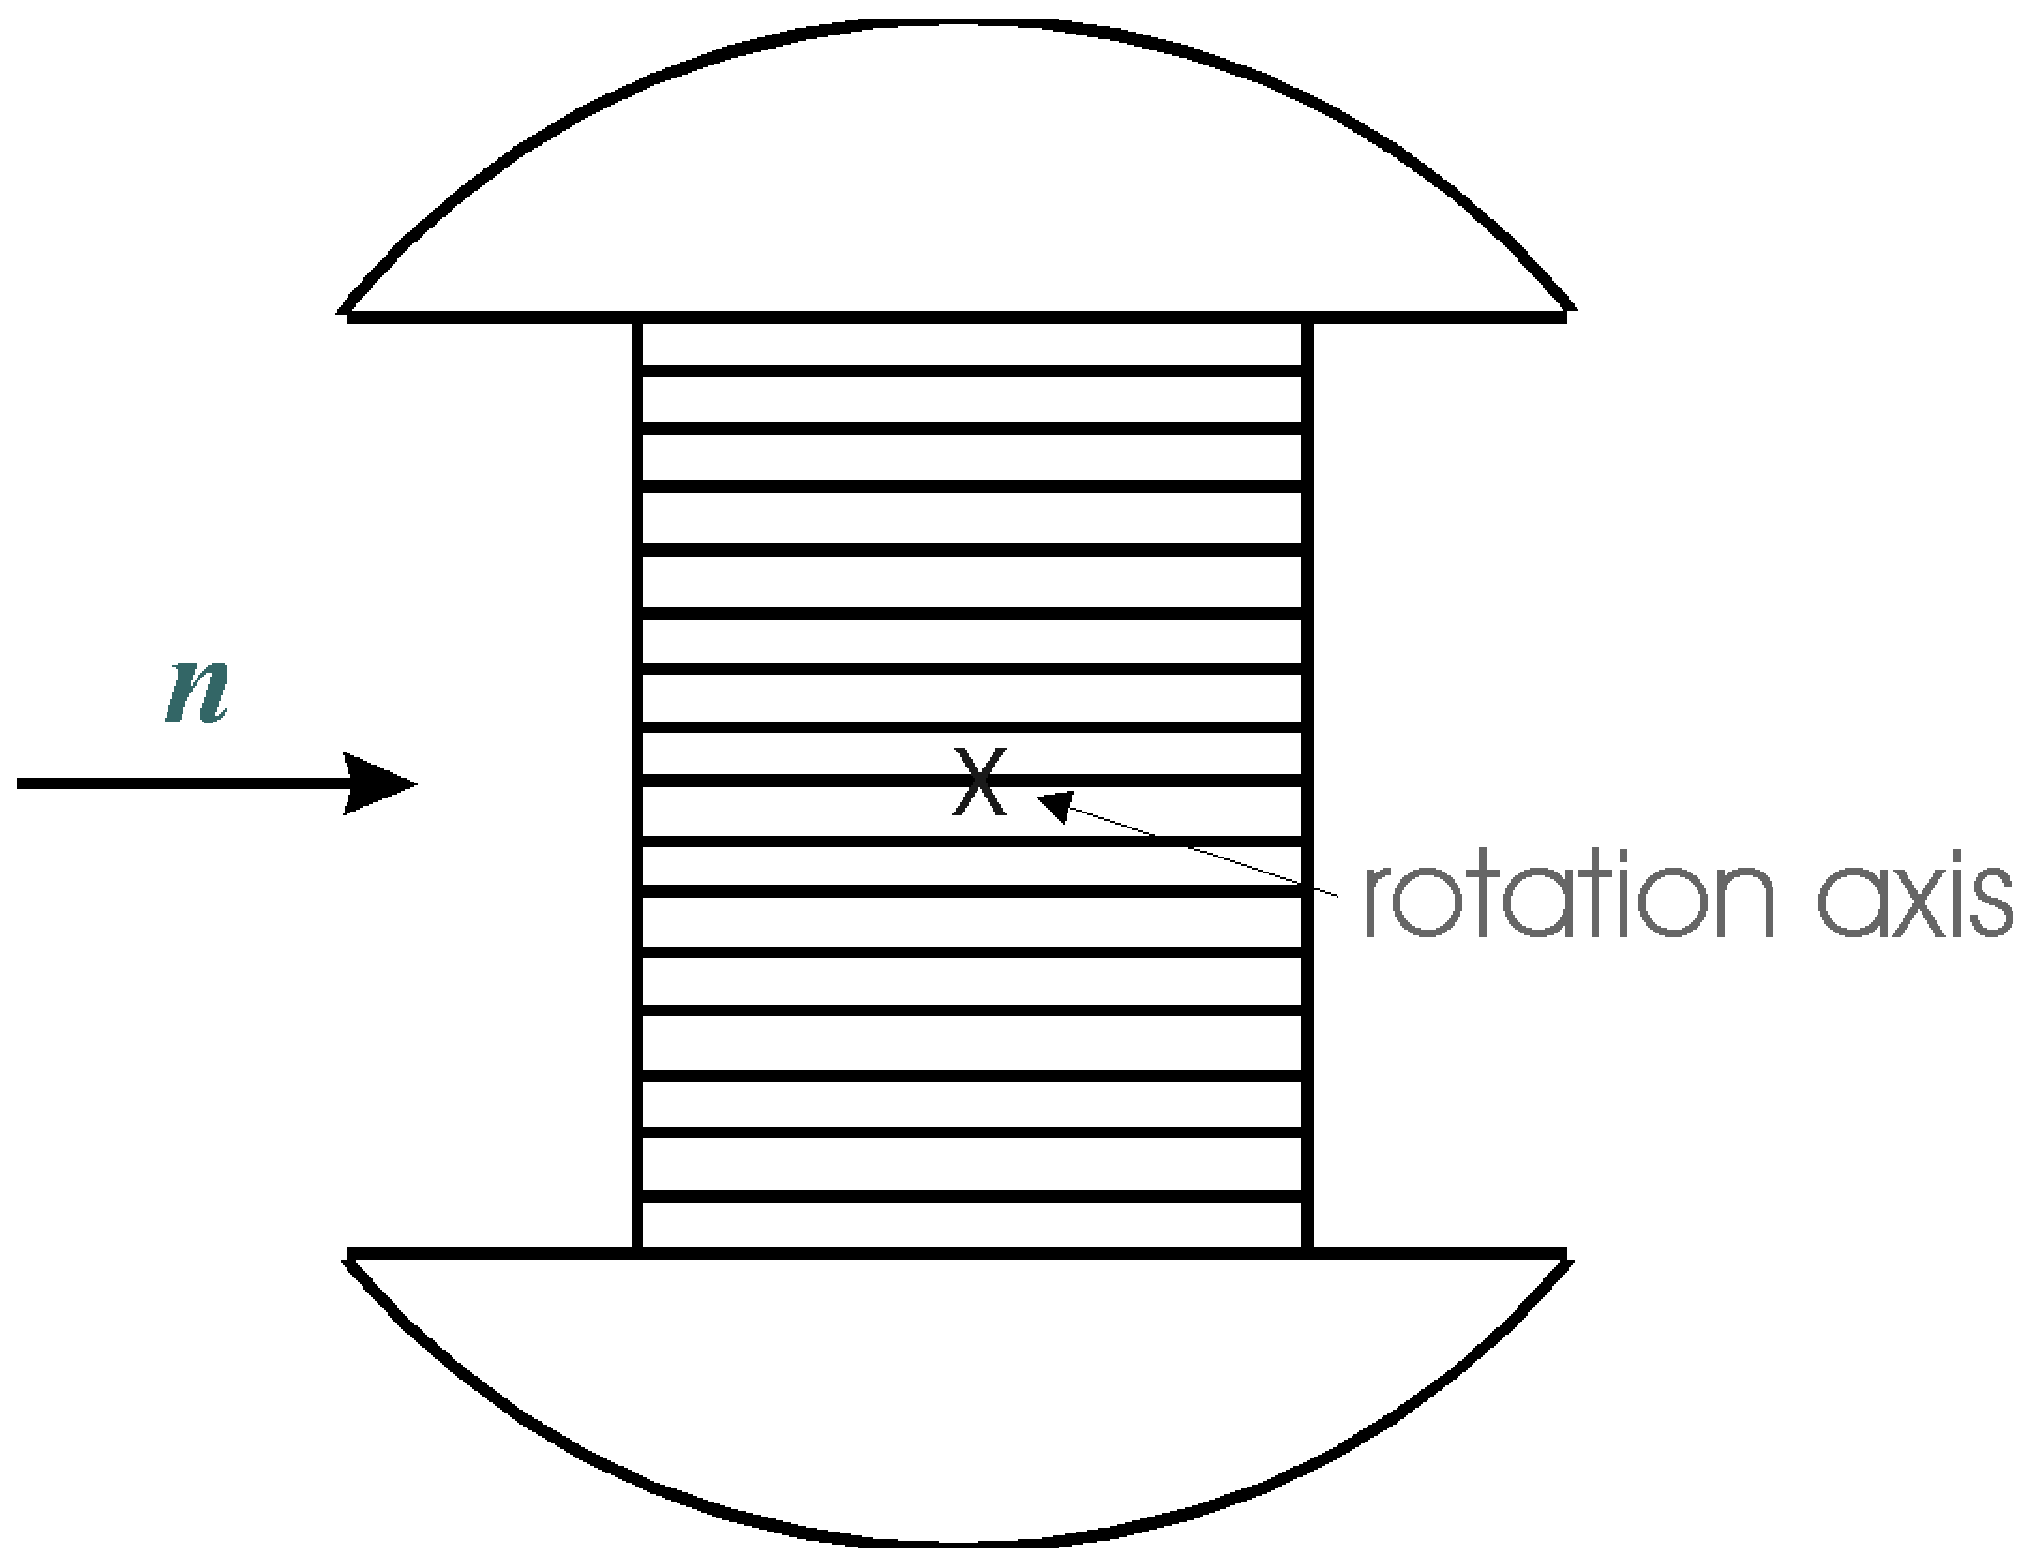
\includegraphics[width=0.45\linewidth]{figures/vitess_fc_str.eps}
\caption{geometry of a staight Fermi chopper\label{f:vit_fc1}}
\end{center}
\end{figure}

Geometry for {\bf parabolic} channels:
In this case, the Fermi chopper is supposed to be a full cylinder, i.e. the central
channels are longer than those on the edges. The other features are the same as for
the other options. (see figure~\ref{f:vit_fc2}).

\begin{figure}[ht]
\begin{center}
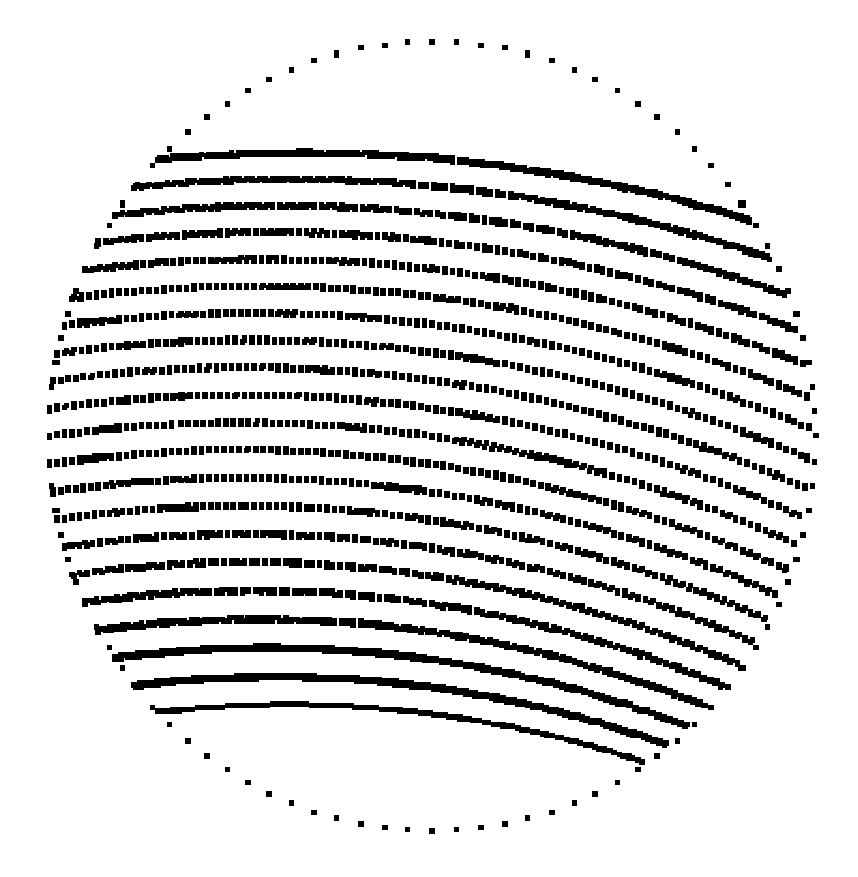
\includegraphics[width=0.4\linewidth]{figures/vitess_fc_parab.eps}
\caption{geometry of a curved Fermi chopper\label{f:vit_fc2}}
\end{center}
\end{figure}

The algorithm works with a rotating chopper framework. Neutrons hitting the channel
walls are absorbed. The channels are approximated by $N_{\rm gates}$ gates. If the trajectory
takes a course through all the gates, the neutron passes the Fermi chopper. There are gates at
the entrance and the exit of the channel. The other gates are situated close to the centre of
the Fermic chopper.
Precision of the simulation increases with the number of gates, but also the computing time needed.
The use of four channels already gives exact transmission shapes for lower wavelengths
($\lambda < 6$ \AA) and good approximation for higher ones. It is recommended to use larger number of
channels only for a check.

The option 'zerotime' may be used to reset the time at the chopper position. The time is
set to a value between -$T_{\rm p}$/2 and +$T_{\rm p}$/2 (with $T_{\rm p}$ being the maximal pulse length),
depending on the phase of the chopper at the moment of passing the chopper centre. The
result is the generation of only 1 pulse instead of several; this is useful for TOF instruments
on continuous sources.

This component is about twice slower than the \verb+FermiChopper+ component.

The component must be placed after a component which sets a non zero flight path to the Fermi Chopper (e.g. not an Arm).

\newpage
\input{optics/V_selector}
\input{optics/Selector}

% there follows a chapter
\newpage
% Emacs settings: -*-mode: latex; TeX-master: "manual.tex"; -*-

\chapter{Monochromators}

In this class of components, we are concerned with elastic Bragg
scattering from monochromators. {\bf Monochromator\_flat}
models a flat thin mosaic crystal with a single scattering vector
perpendicular to the surface.
The component {\bf Monochromator\_curved} is physically similar,
but models a singly or doubly bend monochromator crystal arrangement.

A much more general model of scattering from a single crystal is
found in the component {\bf Single\_crystal},
which is presented under Samples, chapter~\ref{c:samples}.

\section{Monochromator\_flat: An infinitely thin, flat mosaic crystal with
a single scattering vector}
\label{s:monochromator_flat}
\index{Optics!Monochromator}

\component{Monochromator\_flat}{System}{$z_{\rm min}$, $z_{\rm max}$, $y_{\rm min}$, $y_{\rm max}$, $\eta_{\rm h}$, $\eta_{\rm v}$, $R_0$, $Q_0$}{$d_{\rm m}$}{In reflecting geometry, non polarized}

This component simulates an infinitely thin single
crystal with a single scattering vector, $Q_0=2\pi / d_m$, perpendicular to the
surface. A typical
use for this component is to simulate a simple monochromator or analyzer.

The monochromator dimensions are given by the length, $z_{\rm w}$, and
the height, $y_{\rm h}$. As the parameter names indicate, the
monochromator is placed in the $z-y$ plane of the local coordinate system.
This definition is made to ensure that the physical monochromator angle
(often denoted \verb+A1+) will equal the \MCS rotation angle
of the Monochromator component around the $y$-axis.
$R_0$ is the maximal reflectivity and
$\eta_{\rm h}$ and $\eta_{\rm v}$ are the horizontal and vertical mosaicities,
respectively, see explanation below.

\subsection{Monochromator physics and algorithm}
The physical model used in {\bf Monochromator\_flat} is a rectangular piece of
material composed of a large number of small micro-crystals.
The orientation of the
micro-crystals deviates from the nominal crystal orientation so that the
probability of a given micro-crystal orientation is proportional to a
Gaussian in the angle between the given and the nominal orientation. The
width of the Gaussian is given by the mosaic spread, $\eta$, of the crystal
(given in units of arc minutes).
$\eta$ is assumed to be large compared to the inherent Bragg width of the
scattering vector (often a few arc seconds).
(The mosaicity gives rise to a Gaussian reflectivity profile of width
similar to - but not equal - the intrinsic mosaicity.
In this component, and in real life, the mosaicity given is that of the
reflectivity signal.)

As a further simplification, the crystal is assumed to be infinitely
thin. This means that multiple scattering effects are not simulated. It
also means that the total reflectivity, $r_0$ is used as a parameter for
the model rather than the atomic scattering cross section, implying that
the scattering efficiency does not vary with neutron wavelength.
The variance
of the lattice spacing ($\Delta d/d$) is assumed to be zero, so this
component is not suitable for simulating backscattering instruments (use
the component {\rm Single\_crystal}
in section~\ref{s:Single_crystal} for that).

When a neutron trajectory intersects the crystal, the first step in the
computation is to determine the probability of scattering. This
probability is then used in a Monte Carlo choice deciding whether to
scatter or transmit the neutron. The physical scattering probability is the sum
of the probabilities of first- second-, and higher-order scattering -
up to the highest order possible for the given neutron wavelength.
However, in most cases at most one order will have a
significant scattering probability, and the computation thus considers
only the order that best matches the neutron wavelength.

The scattering of neutrons from a crystal is governed by Bragg's law:
\begin{equation}
n{\bf Q}_0 = 2{\bf k}_i\sin\theta
\end{equation}
The scattering order is specified by the integer $n$. We seek only one
value of $n$, namely the one which makes
$n {\bf Q}_0$ closest to the projection of $2{\bf k}_i$ onto ${\bf Q}_0$
(see figure~\ref{f:mosaic_order}).
%  k=2PI/lambda
%  q=2k sin(theta)
%
%  2 PI n/k = d q/2k
%  q = n 4 PI/d
%
%  n 2PI/k = n 4 PI/q \sin\theta
%  1/k = 2/q\sin\theta
%  n q = 2k\sin\theta
\begin{figure}
  \begin{center}
    \psfrag{theta}[l][l]{$\theta$}
    \psfrag{ki}[r][r]{$2{\bf k}_{\rm i}$}
    \psfrag{Q0}[l][l]{${\bf Q}_0$}
    \psfrag{2Q0}[l][l]{$2{\bf Q}_0$}
    \psfrag{3Q0}[l][l]{$3{\bf Q}_0$}
    \psfrag{4Q0}[l][l]{$4{\bf Q}_0$}
    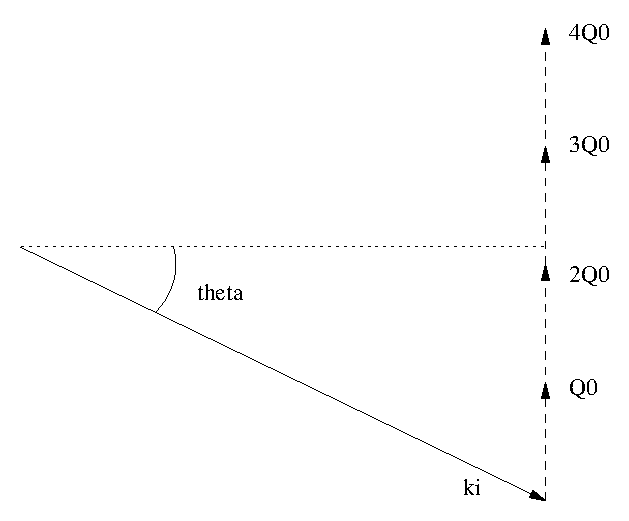
\includegraphics[width=0.5\textwidth]{figures/mosaic_order.eps}
  \end{center}
\caption{Selection of the Bragg order (``2'' in this case).}
\label{f:mosaic_order}
\end{figure}
%

Once $n$ has been determined, the Bragg angle $\theta$ can be
computed. The angle $\alpha$ is the amount one would need to
turn the nominal scattering vector ${\bf Q}_0$ for the monochromator
to be in Bragg scattering condition.
We now use $\alpha$ to compute the probability of reflection from
the mosaic crystal
\begin{equation}
p_{\rm reflect} = R_0 e^{-\alpha^2/2\eta^2},
\end{equation}
The probability $p_{\rm reflect}$ is used
in a Monte Carlo choice to decide whether the neutron is transmitted or
reflected.
%
%\begin{figure}
%  \begin{center}
%    \psfrag{th}[r][r]{$\theta$}
%    \psfrag{ki}[r][r]{$2{\bf k}_{\rm i}$}
%    \psfrag{kf}[l][l]{$2{\bf k}_{\rm f}$}
%    \psfrag{Q0}[l][l]{${\bf Q}_0$}
%    \psfrag{alpha}[c][c]{$\alpha$}
%    \psfrag{q}[l][l]{$\bf q$}
%    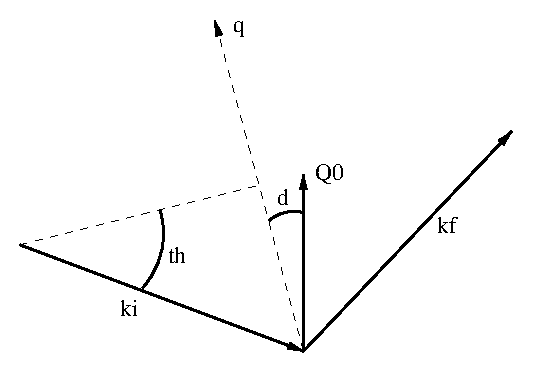
\includegraphics[width=0.5\textwidth]{figures/mosaic_angle.eps}
%  \end{center}
%\caption{Computing the deviation $d$ from the nominal scattering direction.}
%\label{f:mosaic_angle}
%\end{figure}

In the case of reflection, the neutron will be scattered into the
Debye-Scherrer cone, with the probability of each point on the cone
being determined by the mosaic. The Debye-Scherrer cone can be described
by the equation
\begin{equation}
  \label{eq:mosaic_cone}
  {\bf k}_{\rm f} = {\bf k}_{\rm i}\cos2\theta +
      \sin2\theta({\bf c}\cos\varphi + {\bf b}\sin\varphi),
      \qquad\varphi\in[-\pi;\pi],
\end{equation}
where ${\bf b}$ is a vector perpendicular to ${\bf k}_{\rm i}$ and ${\bf
Q}_0$, ${\bf c}$ is perpendicular to ${\bf k}_{\rm i}$ and ${\bf b}$,
and both ${\bf b}$ and ${\bf c}$ have the same length as ${\bf k}_{\rm i}$
(see figure~\ref{f:mosaic_cone}). When choosing $\varphi$ (and
thereby ${\bf k}_{\rm f}$), only a small part of the full $[-\pi; \pi]$
range will have appreciable scattering probability in non-backscattering
configurations. The best statistics is thus obtained by sampling
$\varphi$ only from a suitably narrow range.

The (small) deviation angle $\alpha$ of the nominal
scattering vector $n{\bf Q}_0$ corresponds to a $\Delta q$ of
\begin{equation}
\Delta q \approx \alpha 2k\sin\theta.
\end{equation}
The angle $\varphi$ corresponds to a $\Delta k_{\rm f}$ (and hence
$\Delta q$) of
\begin{equation}
\Delta q \approx \varphi k \sin(2\theta)
\end{equation}
(see figure~\ref{f:mosaic_cone}).
Hence we may sample $\varphi$ from a Gaussian with standard deviation
\begin{equation}
\alpha\frac{2k\sin\theta}{k\sin(2\theta)} =
\alpha\frac{2k\sin\theta}{2k\sin\theta\cos\theta} =
\frac{\alpha}{\cos\theta}
\end{equation}
to get good statistics.
%
\begin{figure}
  \begin{center}
    \psfrag{th}[r][r]{$2\theta$}
    \psfrag{ki}[c][c]{$2{\bf k}_{\rm i}$}
    \psfrag{kf}[r][r]{$2{\bf k}_{\rm f}$}
    \psfrag{nQ0}[l][l]{$n{\bf Q}_0$}
    \psfrag{q}[l][l]{$\bf q$}
    \psfrag{2ksin2t}[l][l]{$2 k \sin(2 \theta)$}
    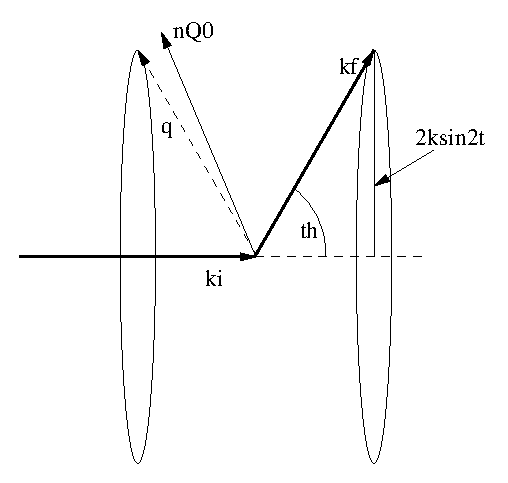
\includegraphics[width=0.5\textwidth]{figures/mosaic_cone.eps}
  \end{center}
\caption{Scattering into the part of the Debye-Scherrer cone covered by
    the mosaic.}
\label{f:mosaic_cone}
\end{figure}

What remains is to determine the neutron weight. The distribution from
which the scattering event is sampled is a Gaussian in $\varphi$ of
width $\frac{\alpha}{\cos\theta}$,
\begin{equation}
    f_{\rm MC}(\varphi) = \frac{1}{\sqrt{2\pi}(\sigma/\cos\theta)}
            e^{-\varphi^2/2(\sigma/\cos\theta)^2}
\end{equation}
In the physical model, the probability of the scattering event is
proportional to a Gaussian in the angle between the nominal scattering
vector ${\bf Q}_0$ and the actual scattering vector ${\bf q}$. The
normalization condition is that the integral over all $\varphi$ should
be 1. Thus the probability of the scattering event in the physical model
is
\begin{equation}
  \label{eq:mosaic_integral}
  \Pi(\varphi) = e^{\frac{-d(\varphi)^2}{2\sigma^2}} /
   \int_{-\pi}^{\pi} e^{\frac{-d(\varphi)^2}{2\sigma^2}} d\varphi
\end{equation}
where $d(\varphi)$ denotes the angle between the nominal scattering
vector and the actual scattering vector corresponding to $\varphi$.
According to equation~(\ref{probrule}), the weight adjustment $\pi_j$ is
then given by
\begin{equation}
\pi_j = \Pi(\varphi) / f_{\rm MC}(\varphi).
\end{equation}
In the implementation, the integral in~(\ref{eq:mosaic_integral}) is computed
using a 15-order Gaussian quadrature formula, with the integral
restricted to an interval of width $5\sigma/\cos\theta$ for the same
reasons discussed above on the sampling of $\varphi$.


\section{Monochromator\_curved: A curved mosaic crystal with
a single scattering vector}
\label{s:monochromator_curved}
\index{Optics!Monochromator, curved}

\component{Monochromator\_curved}{(System) Peter Link, FRM-2}{$z_{\rm w}$, $y_{\rm h}$, gap, $\eta_{\rm h}$, $\eta_{\rm v}$, $n_{\rm h}$, $n_{\rm v}$, $R_0$, $Q$, $r_{\rm h}$, $r_{\rm v}$}{$d_{\rm m}$, $\eta$, $h$, $w$, verbose, transmit, reflect}{In reflecting geometry, non polarized}

\begin{figure}
  \begin{center}
    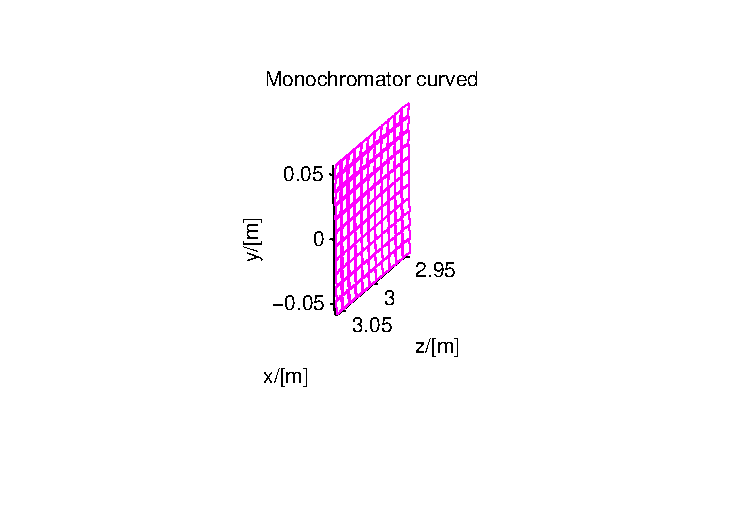
\includegraphics[width=0.9\textwidth]{figures/monochromator_curved.eps}
  \end{center}
\caption{A curved monochromator}
\label{f:monochromator_curved}
\end{figure}


This component simulates an array of infinitely thin single
crystals with a single scattering vector perpendicular to the
surface and a mosaic spread.
This component is used to simulate a singly or doubly
curved monochromator or analyzer in reflecting geometry.

The component uses rectangular pieces of monochromator material
as described in {\bf Monochromator\_curved}.
The scattering vector is named $Q$, and as described in
{\bf Monochromator\_flat}, multiples of $Q$ will be applied.
Other important parameters are the piece height and width,
$y_{\rm h}$ and $z_{\rm w}$, respectively, the
horizontal and vertical mosaicities, $\eta_{\rm h}$ and $\eta_{\rm v}$,
respectively.
If just one mosaicity, $\eta$, is specified, this the same for both directions.

The number of pieces vertically and horizontally are called
$n_{\rm v}$ and $n_{\rm h}$, respectively, and the vertical and horizontal
radii of curvature are named $r_{\rm v}$ and $r_{\rm h}$, respectively.
All single crystals are positioned in the same vertical plane,
but tilted accordingly to the curvature radius.

The constant monochromator reflectivity, $R_0$ can be replaced by
a file of tabulated reflectivities $reflect$ (\verb+*.rfl+ in \verb+MCSTAS/data+). In the same sense, the transmission
can be modeled by a tabulated file $transmit$ (for non-reflected neutrons, \verb+*.trm+ in \verb+MCSTAS/data+).
The most useful of these files for Monochromator\_curved are \verb+HOPG.rlf+ and \verb+HOPG.trm+.

As for {\bf Monochromator\_flat}, the crystal is assumed to be infinitely
thin, and the variation in lattice spacing, ($\Delta d/d$),
is assumed to be zero. Hence, this
component is not suitable for simulating backscattering instruments or to
investigate multiple scattering effects.

The theory and algorithm for scattering from
the individual blades is described under {\bf Monochromator\_flat}.


\section{Single\_crystal: Thick single crystal monochromator plate with multiple scattering}
\index{Optics!Monochromator, thick}

The {\bf Single\_crystal} component may be used to study more complex monochromators, including incoherent scattering, thickness and multiple scattering. Please refer to section \ref{s:Single_crystal}.

\section{Phase space transformer - moving monochromator}
\index{Optics!phase space transformer}

Eventhough there exist a few attempts to write dedicated phase space transformer components, there is an elegant way to put a monochromator into move, by mean of the EXTEND keyword. If you define a SPEED parameter for the instrument, the idea is to change the coordinate system before the monochromator, and restore it afterwards, as follow in the TRACE section:
\begin{verbatim}
DEFINE INSTRUMENT PST(SPEED=200, ...)
(...)
TRACE
(...)
COMPONENT Mono_PST_on=Arm()
AT ...
EXTEND %{
  vx = vx + SPEED; // monochromator moves transversaly by SPPED m/s
%}

COMPONENT  Mono=Monochromator(...)
AT (0,0,0) RELATIVE PREVIOUS

COMPONENT Mono_PST_off=Arm
AT (0,0,0) RELATIVE PREVIOUS
EXTEND  %{
  vz = vz - SPEED; // puts back neutron in static coordinate frame
%}
\end{verbatim}
This solution does not contain acceleration, but is far enough for most
studies, and it is very simple. In the latter example, the instance \verb+Mono_PST_on+ should itself be rotated to reflect according to a Bragg law.

